% Preview body


\section{Aula 3}


\subsection{Introdução ao problema de fluxo de potência}

Como os elementos vistos na aula anterior se combinam, formando um
sistema elétrico. Objetivo apresentar as equações de fluxo de potência 

Introduziremos a seguir os conceitos das leis de Kirchoff, que valem
tanto para circuitos pequenos como para sistemas elétricos inteiros.
A\textbf{ Primeira Lei de Kirchoff} enuncia que em qualquer nó, a
soma das correntes que deixam este nó (aquelas cujas apontam para
fora do nó) é igual a soma das correntes que chegam até ele. Observe
a figura \ref{fig:Exemplo-de-circuito}, a equação para o nó $a$
para satisfazer a primeira lei de Kirchoff é 
\[
i_{1}+i_{2}=i_{3}.
\]


\begin{figure}
\begin{centering}
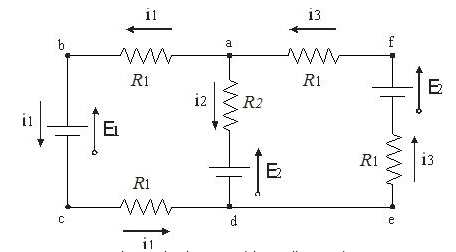
\includegraphics{anexos/aula3_circuito}
\par\end{centering}

\protect\caption{\label{fig:Exemplo-de-circuito}Exemplo de circuito}
\end{figure}


Já a \textbf{Segunda Lei de Kirchoff} estabelece que a soma algébrica
das forças eletromotrizes (f.e.m) em qualquer malha é igual a soma
algébrica, considerando os sentidos, das quedas de tensão (ou dos
produtos $i\cdot R$) contidos na malha. Observando a malha da esquerda
do circuito apresentado na figura \ref{fig:Exemplo-de-circuito},
essa lei equivale a equação
\[
E_{1}+R_{1}\cdot i_{1}-R_{2}\cdot i_{2}-E_{2}+R_{1}\cdot i_{1}=0.
\]


Para modelar a rede, considera-se um modelo em que as fontes de tensão
foram transformadas em fontes de corrente em paralelo. %
\begin{comment}
VERIFICAR
\end{comment}


A figura \ref{fig:modelagem-sistema} mostra um diagrama da representação
de um sistema elétrico como um circuito, cujos elementos são impedâncias
(ou admitâncias, que é o inverso da impedância). Esse sistema pode
ser modelado com as seguintes equações:

\[
\begin{aligned}\dot{I}_{k}=\dot{I}_{km}+\dot{I}_{km}^{sh}, & (\mbox{Corrente injetada na barra \ensuremath{k})}\\
\dot{I}_{m}=\dot{I}_{mk}+\dot{I}_{mk}^{sh}, & (\mbox{Corrente injetada na barra \ensuremath{m})}\\
y_{km}=\frac{1}{R_{km}+jx_{km}}, & (\mbox{Admitância da linha)}\\
\dot{I}_{km}=(\dot{V}_{k}-\dot{V}_{m})\cdot y_{km}, & (\mbox{Corrente na linha)}\\
\dot{I}_{km}^{sh}=j\cdot\dot{V}_{k}\cdot b_{km}^{sh}, & (\mbox{Corrente no ramo shunt)}\\
\dot{I}_{km}=(\dot{V}_{k}-\dot{V}_{m})\cdot y_{km}, & (\mbox{Corrente na linha)}\\
\dot{I}_{km}^{sh}=j\cdot\dot{V}_{k}\cdot b_{km}^{sh}, & (\mbox{Corrente injetada na barra \ensuremath{m})}
\end{aligned}
\]


\begin{comment}
Ramo shunt. Que é? É tipo terra?
\end{comment}


\begin{figure}
\begin{centering}
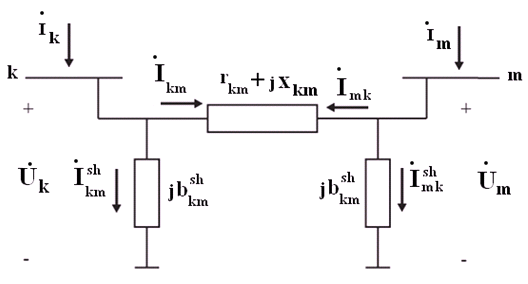
\includegraphics{anexos/aula3_circuito2}
\par\end{centering}

\protect\caption{\label{fig:modelagem-sistema}Exemplo de modelagem de linha de transmissão}
\end{figure}


Matematicamente, as correntes injetadas nas barras podem ser obtidas
por:

\[
\left[\begin{array}{c}
i_{k}\\
i_{m}
\end{array}\right]=\left[\begin{array}{cc}
y_{km}+jb_{km}^{sh} & -y_{km}\\
-y_{km} & y_{km}+jb_{km}^{sh}
\end{array}\right]\left[\begin{array}{c}
\dot{V}_{k}\\
\dot{V}_{m}
\end{array}\right]\quad\longrightarrow\quad I=\left[Y_{bus}\right]\cdot U,
\]
em que $I$ representa o vetor de corrente nodal e $U$ o vetor de
tensão nodal. A regra da formação da matriz $Y_{bus}$ são:
\[
Y_{kk}=\sum_{m=1}^{n}\left(y_{km}+jb_{km}^{sh}\right)
\]


\[
Y_{km}=-y_{km}
\]
em que $Y$ é a matriz de admitância de barra e $n$ o número de barras
do sistema. Utiliza-se como notação a letra maiúscula com índice duplo
($Y_{kk},$ por exemplo) para representar um elemento da matriz $Y$,
enquanto a letra minúscula com índice duplo ($y_{km},$ e.g.) representa
a admitância do elemento do sistema. 

Assim, para um sistema de $n$ barras, matriz $Y_{bus}$ pode ser
escrita da seguinte forma:

\[
\left[Y_{bus}\right]=\left[\begin{array}{ccc}
Y_{11} & \cdots & Y_{1n}\\
\vdots & \ddots & \vdots\\
Y_{n1} & \cdots & Y_{nn}
\end{array}\right]=\left[\begin{array}{ccc}
G_{11}+jB_{11} & \cdots & G_{1n}+jB_{1n}\\
\vdots & \ddots & \vdots\\
G_{n1}+jB_{n1} & \cdots & G_{nn}+jB_{nn}
\end{array}\right]
\]
\[
\left[Y_{bus}\right]=\left[\begin{array}{ccc}
G_{11} & \cdots & G_{1n}\\
\vdots & \ddots & \vdots\\
G_{n1} & \cdots & G_{nn}
\end{array}\right]+j\left[\begin{array}{ccc}
B_{11} & \cdots & B_{1n}\\
\vdots & \ddots & \vdots\\
B_{n1} & \cdots & B_{nn}
\end{array}\right],
\]
em que $G$ é a matriz de condutância nodal e $B$ a matriz de suceptância
nodal.

A potência complexa injetada em uma barra é dada por 

\begin{equation}
S_{k}=\dot{V}_{k}\cdot\dot{I}_{k}^{*},\label{eq:aula3_sk}
\end{equation}
em que 
\begin{equation}
\dot{I}_{k}=\sum_{m=1}^{n}Y_{km}\cdot\dot{V}.\label{eq:aula3_iksum}
\end{equation}
Substituindo \ref{eq:aula3_iksum} em \ref{eq:aula3_sk}, obtemos
que 
\[
S_{k}=\dot{V}_{k}\cdot\left(\dot{I}_{k}=\sum_{m=1}^{n}Y_{km}\cdot\dot{V}\right)^{*}.
\]
Reescrevendo através de fasores obtemos que

\[
\begin{aligned}S_{k} & =V_{k}\angle\theta_{k}\cdot\left[\sum_{m=1}^{n}(G_{km}+jB_{km})\cdot V_{m}\angle\theta_{m}\right]^{*}\\
 & =V_{k}\angle\theta_{k}\cdot\left[\sum_{m=1}^{n}(G_{km}-jB_{km})\cdot V_{m}\angle-\theta_{m}\right]\\
 & =\left[\sum_{m=1}^{n}(G_{km}-jB_{km})\cdot V_{k}\cdot V_{m}\angle\underbrace{\theta_{k}-\theta_{m}}_{\mbox{chamando de \ensuremath{\theta_{km}}}}\right]\\
 & =\left[\sum_{m=1}^{n}\underbrace{G_{km}\cdot V_{k}\cdot V_{m}\angle\theta_{km}}_{G'}-\underbrace{jB_{km}\cdot V_{k}\cdot V_{m}\angle\theta_{km}}_{B'}\right]
\end{aligned}
\]
\begin{comment}
24:16
\end{comment}
A potência injetada em uma barra é dada também por 
\[
S_{k}=P_{k}+jQ_{k}.
\]
$P_{k},$ o componente real, chamado de parte da potência ativa, é
aquele que realiza trabalho no sistema, que acende lâmpadas, fornece
energia para motores, etc. Já $Q_{k}$, o componente imaginário, chamado
de parte reativa, é aquela que sustenta o sistema, mantendo os níveis
de tensão. As equações das potências injetadas em cada barra $k$
são dadas por
\[
\begin{aligned}P_{k} & =V_{k}\sum_{m=1}^{n}V_{m}\cdot(G_{km}\cdot\cos\,\theta_{km}+B_{km}\cdot\sin\,\theta_{km}),\qquad\forall k=1,\dots,n\\
Q_{k} & =V_{k}\sum_{m=1}^{n}V_{m}\cdot(G_{km}\cdot\cos\,\theta_{km}-B_{km}\cdot\sin\,\theta_{km}),\qquad\forall k=1,\dots,n
\end{aligned}
\]
Assim, para cada barra temos 2 equações, o que gera um total de $2n$
equações para todo o sistema, em que as variáveis podem ser $P_{k}$,
$Q_{k}$, $\theta_{k}$ e $V_{k}$. $G_{k}$ é um parâmetro que varia
de acordo com o tipo de linha tratado e $V_{k}$, que representa a
magnitude da potência.%
\begin{comment}
\end{comment}


As barras do sistema elétrico podem ter seus valores fixos ou estarem
soltos para que se ajustem às restrições impostas pelo fluxo de potência
necessário para que as equações sejam satisfeitas. 

\begin{figure}
\begin{centering}
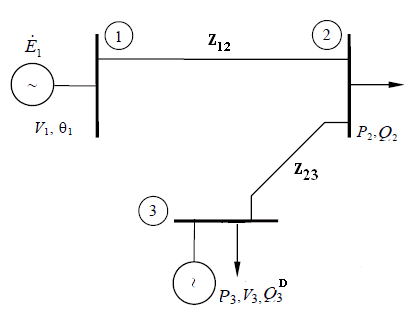
\includegraphics{anexos/aula3_barras}
\par\end{centering}



\protect\caption{\label{fig:modelagem-sistema-1}Exemplo de modelagem de linha de transmissão}
\end{figure}


